% Options for packages loaded elsewhere
\PassOptionsToPackage{unicode}{hyperref}
\PassOptionsToPackage{hyphens}{url}
%
\documentclass[
]{article}
\usepackage{lmodern}
\usepackage{amssymb,amsmath}
\usepackage{ifxetex,ifluatex}
\ifnum 0\ifxetex 1\fi\ifluatex 1\fi=0 % if pdftex
  \usepackage[T1]{fontenc}
  \usepackage[utf8]{inputenc}
  \usepackage{textcomp} % provide euro and other symbols
\else % if luatex or xetex
  \usepackage{unicode-math}
  \defaultfontfeatures{Scale=MatchLowercase}
  \defaultfontfeatures[\rmfamily]{Ligatures=TeX,Scale=1}
\fi
% Use upquote if available, for straight quotes in verbatim environments
\IfFileExists{upquote.sty}{\usepackage{upquote}}{}
\IfFileExists{microtype.sty}{% use microtype if available
  \usepackage[]{microtype}
  \UseMicrotypeSet[protrusion]{basicmath} % disable protrusion for tt fonts
}{}
\makeatletter
\@ifundefined{KOMAClassName}{% if non-KOMA class
  \IfFileExists{parskip.sty}{%
    \usepackage{parskip}
  }{% else
    \setlength{\parindent}{0pt}
    \setlength{\parskip}{6pt plus 2pt minus 1pt}}
}{% if KOMA class
  \KOMAoptions{parskip=half}}
\makeatother
\usepackage{xcolor}
\IfFileExists{xurl.sty}{\usepackage{xurl}}{} % add URL line breaks if available
\IfFileExists{bookmark.sty}{\usepackage{bookmark}}{\usepackage{hyperref}}
\hypersetup{
  pdftitle={DataFest},
  pdfauthor={Albert Sun and Ben Wallace},
  hidelinks,
  pdfcreator={LaTeX via pandoc}}
\urlstyle{same} % disable monospaced font for URLs
\usepackage[margin=1in]{geometry}
\usepackage{color}
\usepackage{fancyvrb}
\newcommand{\VerbBar}{|}
\newcommand{\VERB}{\Verb[commandchars=\\\{\}]}
\DefineVerbatimEnvironment{Highlighting}{Verbatim}{commandchars=\\\{\}}
% Add ',fontsize=\small' for more characters per line
\usepackage{framed}
\definecolor{shadecolor}{RGB}{248,248,248}
\newenvironment{Shaded}{\begin{snugshade}}{\end{snugshade}}
\newcommand{\AlertTok}[1]{\textcolor[rgb]{0.94,0.16,0.16}{#1}}
\newcommand{\AnnotationTok}[1]{\textcolor[rgb]{0.56,0.35,0.01}{\textbf{\textit{#1}}}}
\newcommand{\AttributeTok}[1]{\textcolor[rgb]{0.77,0.63,0.00}{#1}}
\newcommand{\BaseNTok}[1]{\textcolor[rgb]{0.00,0.00,0.81}{#1}}
\newcommand{\BuiltInTok}[1]{#1}
\newcommand{\CharTok}[1]{\textcolor[rgb]{0.31,0.60,0.02}{#1}}
\newcommand{\CommentTok}[1]{\textcolor[rgb]{0.56,0.35,0.01}{\textit{#1}}}
\newcommand{\CommentVarTok}[1]{\textcolor[rgb]{0.56,0.35,0.01}{\textbf{\textit{#1}}}}
\newcommand{\ConstantTok}[1]{\textcolor[rgb]{0.00,0.00,0.00}{#1}}
\newcommand{\ControlFlowTok}[1]{\textcolor[rgb]{0.13,0.29,0.53}{\textbf{#1}}}
\newcommand{\DataTypeTok}[1]{\textcolor[rgb]{0.13,0.29,0.53}{#1}}
\newcommand{\DecValTok}[1]{\textcolor[rgb]{0.00,0.00,0.81}{#1}}
\newcommand{\DocumentationTok}[1]{\textcolor[rgb]{0.56,0.35,0.01}{\textbf{\textit{#1}}}}
\newcommand{\ErrorTok}[1]{\textcolor[rgb]{0.64,0.00,0.00}{\textbf{#1}}}
\newcommand{\ExtensionTok}[1]{#1}
\newcommand{\FloatTok}[1]{\textcolor[rgb]{0.00,0.00,0.81}{#1}}
\newcommand{\FunctionTok}[1]{\textcolor[rgb]{0.00,0.00,0.00}{#1}}
\newcommand{\ImportTok}[1]{#1}
\newcommand{\InformationTok}[1]{\textcolor[rgb]{0.56,0.35,0.01}{\textbf{\textit{#1}}}}
\newcommand{\KeywordTok}[1]{\textcolor[rgb]{0.13,0.29,0.53}{\textbf{#1}}}
\newcommand{\NormalTok}[1]{#1}
\newcommand{\OperatorTok}[1]{\textcolor[rgb]{0.81,0.36,0.00}{\textbf{#1}}}
\newcommand{\OtherTok}[1]{\textcolor[rgb]{0.56,0.35,0.01}{#1}}
\newcommand{\PreprocessorTok}[1]{\textcolor[rgb]{0.56,0.35,0.01}{\textit{#1}}}
\newcommand{\RegionMarkerTok}[1]{#1}
\newcommand{\SpecialCharTok}[1]{\textcolor[rgb]{0.00,0.00,0.00}{#1}}
\newcommand{\SpecialStringTok}[1]{\textcolor[rgb]{0.31,0.60,0.02}{#1}}
\newcommand{\StringTok}[1]{\textcolor[rgb]{0.31,0.60,0.02}{#1}}
\newcommand{\VariableTok}[1]{\textcolor[rgb]{0.00,0.00,0.00}{#1}}
\newcommand{\VerbatimStringTok}[1]{\textcolor[rgb]{0.31,0.60,0.02}{#1}}
\newcommand{\WarningTok}[1]{\textcolor[rgb]{0.56,0.35,0.01}{\textbf{\textit{#1}}}}
\usepackage{graphicx,grffile}
\makeatletter
\def\maxwidth{\ifdim\Gin@nat@width>\linewidth\linewidth\else\Gin@nat@width\fi}
\def\maxheight{\ifdim\Gin@nat@height>\textheight\textheight\else\Gin@nat@height\fi}
\makeatother
% Scale images if necessary, so that they will not overflow the page
% margins by default, and it is still possible to overwrite the defaults
% using explicit options in \includegraphics[width, height, ...]{}
\setkeys{Gin}{width=\maxwidth,height=\maxheight,keepaspectratio}
% Set default figure placement to htbp
\makeatletter
\def\fps@figure{htbp}
\makeatother
\setlength{\emergencystretch}{3em} % prevent overfull lines
\providecommand{\tightlist}{%
  \setlength{\itemsep}{0pt}\setlength{\parskip}{0pt}}
\setcounter{secnumdepth}{-\maxdimen} % remove section numbering

\title{DataFest}
\author{Albert Sun and Ben Wallace}
\date{4/9/2020}

\begin{document}
\maketitle

\begin{Shaded}
\begin{Highlighting}[]
\KeywordTok{library}\NormalTok{(dplyr)}
\end{Highlighting}
\end{Shaded}

\begin{verbatim}
## Warning: package 'dplyr' was built under R version 3.6.2
\end{verbatim}

\begin{verbatim}
## 
## Attaching package: 'dplyr'
\end{verbatim}

\begin{verbatim}
## The following objects are masked from 'package:stats':
## 
##     filter, lag
\end{verbatim}

\begin{verbatim}
## The following objects are masked from 'package:base':
## 
##     intersect, setdiff, setequal, union
\end{verbatim}

\begin{Shaded}
\begin{Highlighting}[]
\KeywordTok{library}\NormalTok{(ggplot2)}
\end{Highlighting}
\end{Shaded}

\begin{verbatim}
## Warning: package 'ggplot2' was built under R version 3.6.2
\end{verbatim}

\begin{Shaded}
\begin{Highlighting}[]
\KeywordTok{library}\NormalTok{(patchwork)}
\end{Highlighting}
\end{Shaded}

\begin{verbatim}
## Warning: package 'patchwork' was built under R version 3.6.3
\end{verbatim}

\begin{Shaded}
\begin{Highlighting}[]
\KeywordTok{library}\NormalTok{(twitteR)}
\end{Highlighting}
\end{Shaded}

\begin{verbatim}
## Warning: package 'twitteR' was built under R version 3.6.3
\end{verbatim}

\begin{verbatim}
## 
## Attaching package: 'twitteR'
\end{verbatim}

\begin{verbatim}
## The following objects are masked from 'package:dplyr':
## 
##     id, location
\end{verbatim}

\begin{Shaded}
\begin{Highlighting}[]
\KeywordTok{library}\NormalTok{(lubridate)}
\end{Highlighting}
\end{Shaded}

\begin{verbatim}
## Warning: package 'lubridate' was built under R version 3.6.2
\end{verbatim}

\begin{verbatim}
## 
## Attaching package: 'lubridate'
\end{verbatim}

\begin{verbatim}
## The following object is masked from 'package:base':
## 
##     date
\end{verbatim}

\begin{Shaded}
\begin{Highlighting}[]
\KeywordTok{library}\NormalTok{(rvest)}
\end{Highlighting}
\end{Shaded}

\begin{verbatim}
## Warning: package 'rvest' was built under R version 3.6.2
\end{verbatim}

\begin{verbatim}
## Loading required package: xml2
\end{verbatim}

\begin{verbatim}
## Warning: package 'xml2' was built under R version 3.6.2
\end{verbatim}

\begin{Shaded}
\begin{Highlighting}[]
\KeywordTok{library}\NormalTok{(sf)}
\end{Highlighting}
\end{Shaded}

\begin{verbatim}
## Warning: package 'sf' was built under R version 3.6.3
\end{verbatim}

\begin{verbatim}
## Linking to GEOS 3.6.1, GDAL 2.2.3, PROJ 4.9.3
\end{verbatim}

\begin{Shaded}
\begin{Highlighting}[]
\KeywordTok{library}\NormalTok{(tidycensus)}
\end{Highlighting}
\end{Shaded}

\begin{verbatim}
## Warning: package 'tidycensus' was built under R version 3.6.3
\end{verbatim}

\begin{Shaded}
\begin{Highlighting}[]
\KeywordTok{library}\NormalTok{(leaflet)}
\end{Highlighting}
\end{Shaded}

\begin{verbatim}
## Warning: package 'leaflet' was built under R version 3.6.3
\end{verbatim}

\begin{Shaded}
\begin{Highlighting}[]
\KeywordTok{library}\NormalTok{(mapview)}
\end{Highlighting}
\end{Shaded}

\begin{verbatim}
## Warning: package 'mapview' was built under R version 3.6.3
\end{verbatim}

\begin{Shaded}
\begin{Highlighting}[]
\NormalTok{counties <-}\StringTok{ }\KeywordTok{read.csv}\NormalTok{(}\StringTok{"datafiles/us-counties.csv"}\NormalTok{)}
\NormalTok{states <-}\StringTok{ }\KeywordTok{read.csv}\NormalTok{(}\StringTok{"datafiles/us-states.csv"}\NormalTok{)}
\NormalTok{measures <-}\StringTok{ }\KeywordTok{read.csv}\NormalTok{(}\StringTok{"datafiles/statedata.csv"}\NormalTok{)}
\NormalTok{global_measures <-}\StringTok{ }\KeywordTok{read.csv}\NormalTok{(}\StringTok{"datafiles/ACAPSGlobalResponse.csv"}\NormalTok{)}
\NormalTok{covidapproval <-}\StringTok{ }\KeywordTok{read.csv}\NormalTok{(}\StringTok{"datafiles/Covidapproval.csv"}\NormalTok{)}
\end{Highlighting}
\end{Shaded}

\begin{Shaded}
\begin{Highlighting}[]
\NormalTok{toptencounties <-}\StringTok{ }\NormalTok{counties }\OperatorTok
\StringTok{  }\KeywordTok{filter}\NormalTok{(date }\OperatorTok{==}\StringTok{ "2020-04-08"}\NormalTok{) }\OperatorTok
\StringTok{  }\KeywordTok{arrange}\NormalTok{(}\KeywordTok{desc}\NormalTok{(cases))}
  
\NormalTok{toptencounties <-}\StringTok{ }\NormalTok{toptencounties[}\DecValTok{1}\OperatorTok{:}\DecValTok{10}\NormalTok{,]}

\NormalTok{toptenstates <-}\StringTok{ }\NormalTok{states }\OperatorTok
\StringTok{  }\KeywordTok{filter}\NormalTok{(date }\OperatorTok{==}\StringTok{ "2020-04-08"}\NormalTok{) }\OperatorTok
\StringTok{  }\KeywordTok{arrange}\NormalTok{(}\KeywordTok{desc}\NormalTok{(cases))}

\NormalTok{toptenstates <-}\StringTok{ }\NormalTok{toptenstates[}\DecValTok{1}\OperatorTok{:}\DecValTok{10}\NormalTok{,]}
\end{Highlighting}
\end{Shaded}

\hypertarget{ny-state-and-county-date}{%
\section{NY State and County Date}\label{ny-state-and-county-date}}

\begin{Shaded}
\begin{Highlighting}[]
\NormalTok{p1 <-}\StringTok{ }\KeywordTok{ggplot}\NormalTok{(}\DataTypeTok{data =}\NormalTok{ toptencounties, }\DataTypeTok{mapping =} \KeywordTok{aes}\NormalTok{(}\DataTypeTok{x =} \KeywordTok{reorder}\NormalTok{(county, cases), }\DataTypeTok{y =}\NormalTok{ cases), }\DataTypeTok{fill=}\KeywordTok{if_else}\NormalTok{(County}\OperatorTok{==}\StringTok{"New York"}\NormalTok{)) }\OperatorTok{+}
\StringTok{  }\KeywordTok{geom_bar}\NormalTok{(}\DataTypeTok{stat =} \StringTok{"identity"}\NormalTok{) }\OperatorTok{+}\StringTok{ }
\StringTok{  }\KeywordTok{labs}\NormalTok{(}\DataTypeTok{title =} \StringTok{"Top 10 Coronavirus counties cases"}\NormalTok{, }
       \DataTypeTok{y =} \StringTok{"Cases"}\NormalTok{, }\DataTypeTok{x =} \StringTok{"County Name"}\NormalTok{) }\OperatorTok{+}\StringTok{ }
\StringTok{  }\KeywordTok{coord_flip}\NormalTok{()}

\NormalTok{p2 <-}\StringTok{ }\KeywordTok{ggplot}\NormalTok{(}\DataTypeTok{data =}\NormalTok{ toptenstates, }\DataTypeTok{mapping =} \KeywordTok{aes}\NormalTok{(}\DataTypeTok{x =} \KeywordTok{reorder}\NormalTok{(state, cases), }\DataTypeTok{y =}\NormalTok{ cases)) }\OperatorTok{+}
\StringTok{  }\KeywordTok{geom_bar}\NormalTok{(}\DataTypeTok{stat =} \StringTok{"identity"}\NormalTok{) }\OperatorTok{+}\StringTok{ }
\StringTok{  }\KeywordTok{labs}\NormalTok{(}\DataTypeTok{title =} \StringTok{"Top 10 Coronavirus states cases"}\NormalTok{, }
       \DataTypeTok{y =} \StringTok{"Cases"}\NormalTok{, }\DataTypeTok{x =} \StringTok{"State Name"}\NormalTok{) }\OperatorTok{+}\StringTok{ }
\StringTok{  }\KeywordTok{coord_flip}\NormalTok{() }

\NormalTok{p1 }\OperatorTok{+}\StringTok{ }\NormalTok{p2}
\end{Highlighting}
\end{Shaded}

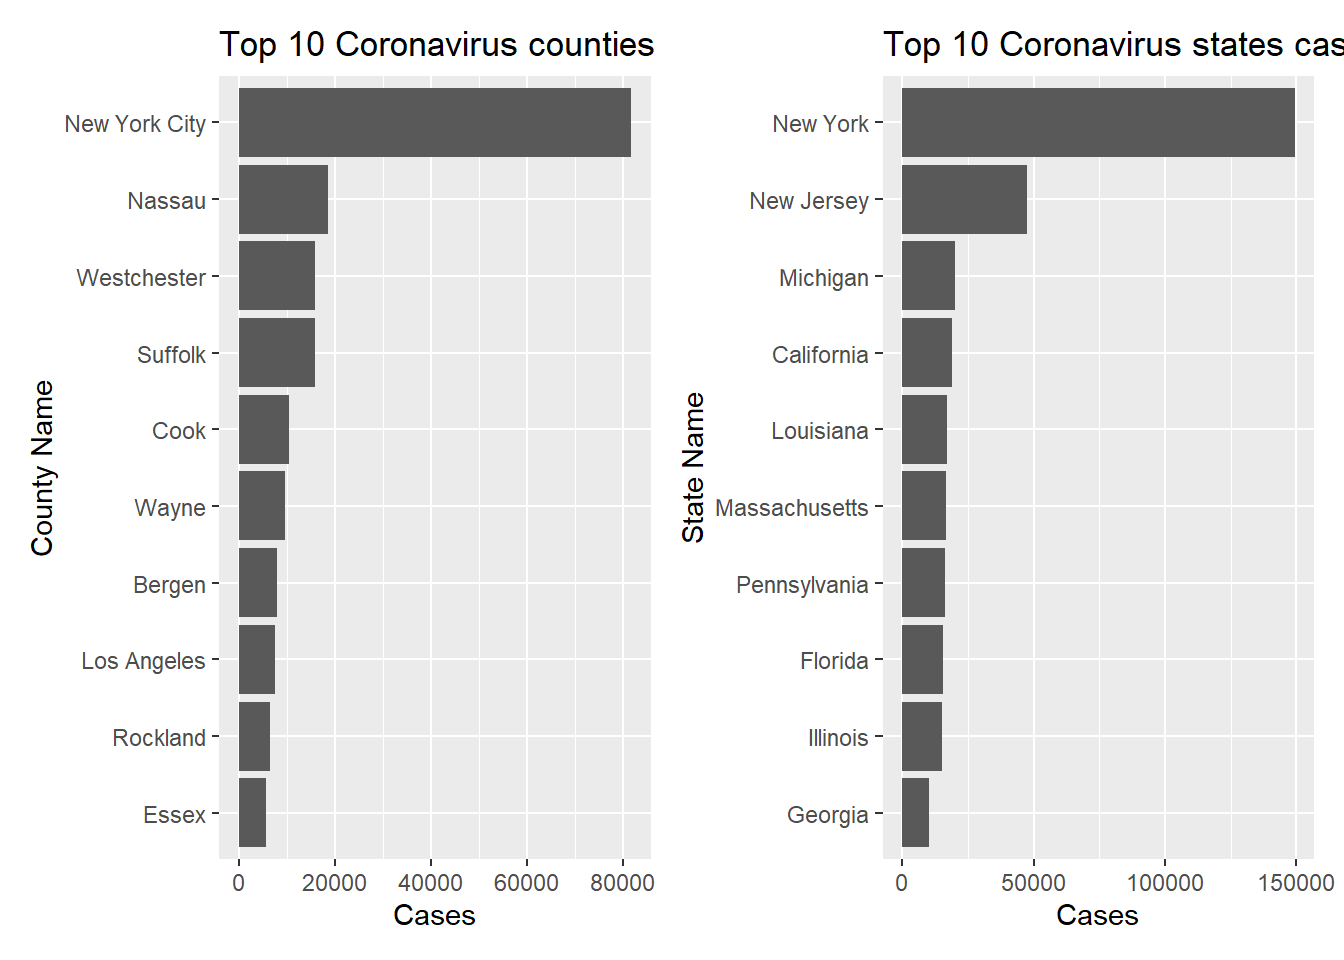
\includegraphics{DataFest_files/figure-latex/plot-1.pdf}

\hypertarget{state-first-stay-at-home}{%
\section{State First Stay at Home}\label{state-first-stay-at-home}}

\begin{Shaded}
\begin{Highlighting}[]
\CommentTok{### Removing United States from df}

\NormalTok{measures <-}\StringTok{ }\NormalTok{measures[}\OperatorTok{-}\KeywordTok{c}\NormalTok{(}\DecValTok{1}\NormalTok{),]}

\NormalTok{dates <-}\StringTok{ }\KeywordTok{c}\NormalTok{(}\StringTok{"4/4/2020 17:00"}\NormalTok{, }\CommentTok{# Dates of stay at home orders}
           \StringTok{"3/28/2020 17:00"}\NormalTok{,}
           \StringTok{"3/31/2020 17:00"}\NormalTok{,}
           \StringTok{""}\NormalTok{,}
           \StringTok{"3/19/2020 0:00"}\NormalTok{,}
           \StringTok{"3/26/2020 6:00"}\NormalTok{,}
           \StringTok{"3/23/2020 20:00"}\NormalTok{,}
           \StringTok{"3/24/2020 8:00"}\NormalTok{,}
           \StringTok{"4/1/2020 0:01"}\NormalTok{,}
           \StringTok{"4/3/2020 0:01"}\NormalTok{,}
           \StringTok{"4/3/2020 0:00"}\NormalTok{,}
           \StringTok{"3/25/2020 0:01"}\NormalTok{,}
           \StringTok{"3/25/2020 13:30"}\NormalTok{,}
           \StringTok{"3/21/2020 17:00"}\NormalTok{,}
           \StringTok{"3/24/2020 23:59"}\NormalTok{,}
           \StringTok{""}\NormalTok{,}
           \StringTok{"3/30/2020 0:01"}\NormalTok{,}
           \StringTok{"3/26/2020 20:00"}\NormalTok{,}
           \StringTok{"3/23/2020 17:00"}\NormalTok{,}
           \StringTok{"4/2/2020 0:01"}\NormalTok{,}
           \StringTok{"3/30/2020 20:00"}\NormalTok{,}
           \StringTok{"3/23/2020 12:00"}\NormalTok{,}
           \StringTok{"3/24/2020 0:01"}\NormalTok{,}
           \StringTok{"3/27/2020 23:59"}\NormalTok{,}
           \StringTok{"4/3/2020 17:00"}\NormalTok{,}
           \StringTok{"4/6/2020 0:01"}\NormalTok{,}
           \StringTok{"3/28/2020 0:01"}\NormalTok{,}
           \StringTok{""}\NormalTok{,}
           \StringTok{"4/1/2020 0:00"}\NormalTok{,}
           \StringTok{"3/27/2020 23:59"}\NormalTok{,}
           \StringTok{"3/21/2020 21:00"}\NormalTok{,}
           \StringTok{"3/24/2020 8:00"}\NormalTok{,}
           \StringTok{"3/22/2020 20:00"}\NormalTok{,}
           \StringTok{"3/30/2020 15:00"}\NormalTok{,}
           \StringTok{""}\NormalTok{,}
           \StringTok{"3/23/2020 23:59"}\NormalTok{,}
           \StringTok{""}\NormalTok{,}
           \StringTok{"3/23/2020 0:00"}\NormalTok{,}
           \StringTok{"4/1/2020 20:00"}\NormalTok{,}
           \StringTok{"3/28/2020 0:00"}\NormalTok{,}
           \StringTok{"4/7/2020 17:00"}\NormalTok{,}
           \StringTok{""}\NormalTok{,}
           \StringTok{"3/31/2020 23:59"}\NormalTok{,}
           \StringTok{"4/2/2020 0:01"}\NormalTok{,}
           \StringTok{""}\NormalTok{,}
           \StringTok{"3/25/2020 17:00"}\NormalTok{,}
           \StringTok{"3/30/2020 0:00"}\NormalTok{,}
           \StringTok{"3/23/2020 0:00"}\NormalTok{,}
           \StringTok{"3/24/2020 20:00"}\NormalTok{,}
           \StringTok{"3/25/2020 8:00"}\NormalTok{,}
           \StringTok{""}
\NormalTok{           )}

\CommentTok{### Adding data to measures df}
\NormalTok{measures <-}\StringTok{ }\NormalTok{measures }\OperatorTok
\StringTok{  }\KeywordTok{mutate}\NormalTok{(}\DataTypeTok{date.stay.at.home =}\NormalTok{ dates)  }\OperatorTok
\StringTok{  }\KeywordTok{mutate}\NormalTok{(}\DataTypeTok{stateno =} \KeywordTok{c}\NormalTok{(}\DecValTok{1}\OperatorTok{:}\DecValTok{51}\NormalTok{))}
\end{Highlighting}
\end{Shaded}

\begin{Shaded}
\begin{Highlighting}[]
\CommentTok{### Plot of stay at home dates}

\NormalTok{measures}\OperatorTok{$}\NormalTok{date.stay.at.home =}\StringTok{ }\KeywordTok{as.Date}\NormalTok{(measures}\OperatorTok{$}\NormalTok{date.stay.at.home, }\StringTok{"%m/%d/%y"}\NormalTok{)}
\NormalTok{med <-}\StringTok{ }\KeywordTok{median}\NormalTok{(measures}\OperatorTok{$}\NormalTok{date.stay.at.home, }\DataTypeTok{na.rm =} \OtherTok{TRUE}\NormalTok{)}
\NormalTok{avg <-}\StringTok{ }\KeywordTok{mean}\NormalTok{(measures}\OperatorTok{$}\NormalTok{date.stay.at.home, }\DataTypeTok{na.rm =} \OtherTok{TRUE}\NormalTok{)}

\KeywordTok{ggplot}\NormalTok{(}\DataTypeTok{data =}\NormalTok{ measures, }\KeywordTok{aes}\NormalTok{(}\DataTypeTok{x =}\NormalTok{ date.stay.at.home)) }\OperatorTok{+}
\StringTok{         }\KeywordTok{geom_histogram}\NormalTok{(}\DataTypeTok{stat =} \StringTok{"count"}\NormalTok{) }\OperatorTok{+}
\StringTok{   }\KeywordTok{scale_x_date}\NormalTok{(}\DataTypeTok{breaks =} \StringTok{"3 days"}\NormalTok{) }\OperatorTok{+}
\StringTok{  }\KeywordTok{theme}\NormalTok{(}\DataTypeTok{axis.text.x =} \KeywordTok{element_text}\NormalTok{(}\DataTypeTok{angle =} \DecValTok{90}\NormalTok{)) }\OperatorTok{+}\StringTok{ }
\StringTok{  }\KeywordTok{geom_vline}\NormalTok{(}\DataTypeTok{xintercept =}\NormalTok{ med, }\DataTypeTok{color =} \StringTok{"darkred"}\NormalTok{) }\OperatorTok{+}
\StringTok{  }\KeywordTok{geom_vline}\NormalTok{(}\DataTypeTok{xintercept =}\NormalTok{ avg, }\DataTypeTok{color =} \StringTok{"navy"}\NormalTok{)}
\end{Highlighting}
\end{Shaded}

\begin{verbatim}
## Warning: Ignoring unknown parameters: binwidth, bins, pad
\end{verbatim}

\begin{verbatim}
## Warning: Removed 8 rows containing non-finite values (stat_count).
\end{verbatim}

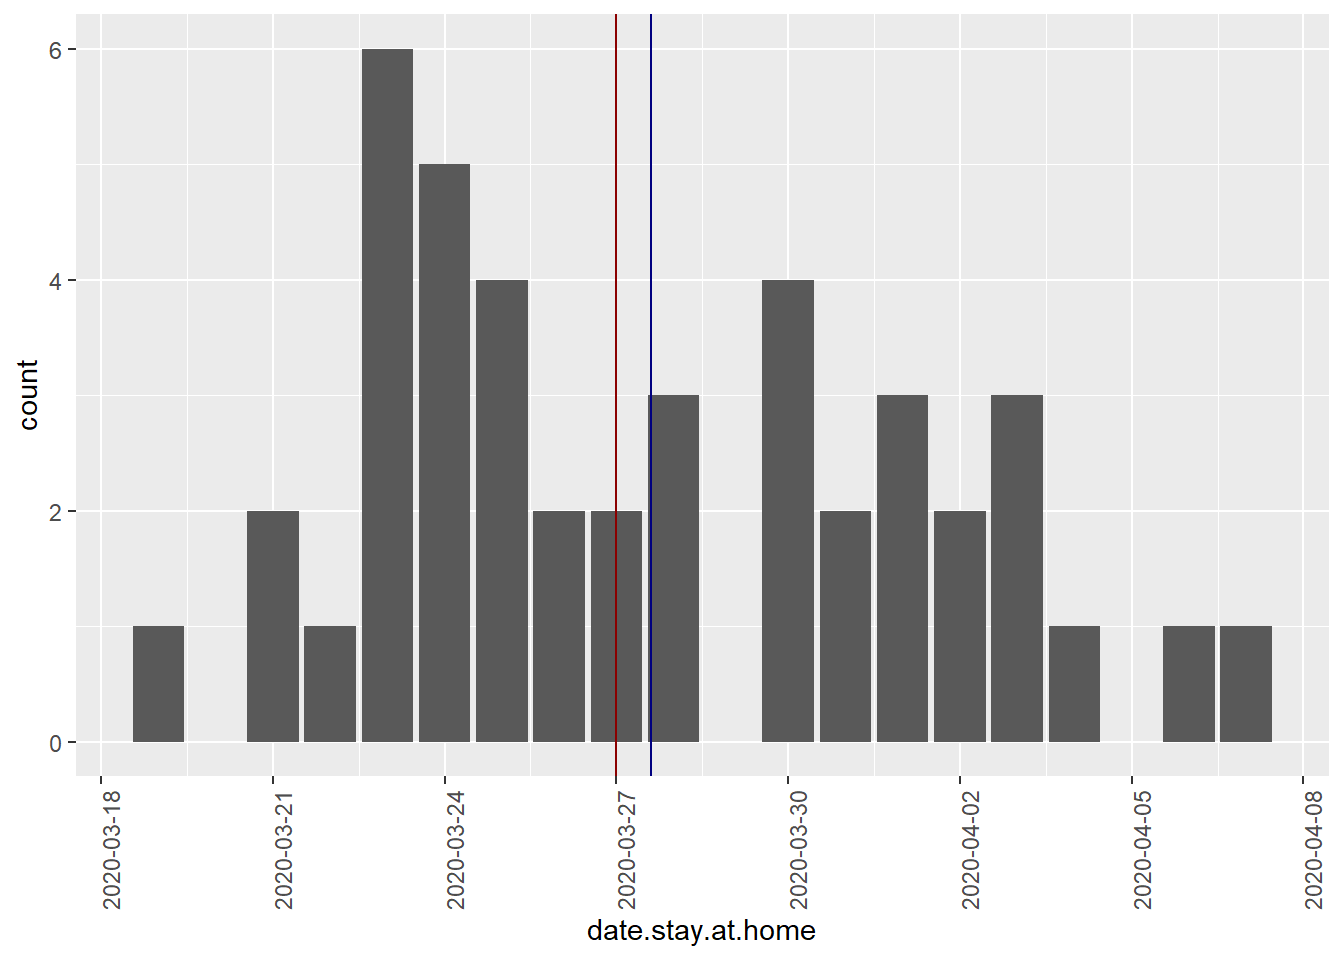
\includegraphics{DataFest_files/figure-latex/plotstayathome-1.pdf}

\hypertarget{twitter}{%
\section{Twitter}\label{twitter}}

TwitteR:

\url{https://opensource.com/article/17/6/collecting-and-mapping-twitter-data-using-r}

\textbf{I'm still applying for a Twitter dev account in order to access
the Twitter API}

\hypertarget{global-measures}{%
\section{Global Measures}\label{global-measures}}

\begin{Shaded}
\begin{Highlighting}[]
\NormalTok{global_measures }\OperatorTok
\StringTok{  }\KeywordTok{filter}\NormalTok{(CATEGORY }\OperatorTok{==}\StringTok{ "Social distancing"}\NormalTok{) }\OperatorTok
\StringTok{  }\KeywordTok{count}\NormalTok{(COUNTRY) }\OperatorTok
\StringTok{  }\KeywordTok{arrange}\NormalTok{(}\OperatorTok{-}\NormalTok{n)}
\end{Highlighting}
\end{Shaded}

\begin{verbatim}
## # A tibble: 173 x 2
##    COUNTRY               n
##    <fct>             <int>
##  1 Ireland              17
##  2 Hungary              14
##  3 Australia            13
##  4 Lithuania            12
##  5 Yemen                12
##  6 Barbados             11
##  7 Czech Republic       11
##  8 Equatorial Guinea    11
##  9 Estonia              11
## 10 Ethiopia             11
## # ... with 163 more rows
\end{verbatim}

First Social Distancing Measure From top-10 quickest and top-10 slowest
Country to test responsiveness:

\begin{Shaded}
\begin{Highlighting}[]
\NormalTok{first_measures <-}\StringTok{ }\NormalTok{global_measures }\OperatorTok
\StringTok{  }\KeywordTok{filter}\NormalTok{(CATEGORY }\OperatorTok{==}\StringTok{ "Social distancing"}\NormalTok{) }\OperatorTok
\StringTok{  }\KeywordTok{mutate}\NormalTok{(}\DataTypeTok{date =} \KeywordTok{dmy}\NormalTok{(DATE_IMPLEMENTED)) }\OperatorTok
\StringTok{  }\KeywordTok{arrange}\NormalTok{(COUNTRY, date) }\OperatorTok
\StringTok{  }\KeywordTok{select}\NormalTok{(COUNTRY, date) }\OperatorTok
\StringTok{  }\KeywordTok{group_by}\NormalTok{(COUNTRY) }\OperatorTok
\StringTok{  }\KeywordTok{slice}\NormalTok{(}\DecValTok{1}\NormalTok{) }\OperatorTok
\StringTok{  }\KeywordTok{ungroup}\NormalTok{() }\OperatorTok
\StringTok{  }\KeywordTok{select}\NormalTok{(COUNTRY, date) }\OperatorTok
\StringTok{  }\KeywordTok{arrange}\NormalTok{(date) }\OperatorTok
\StringTok{  }\KeywordTok{slice}\NormalTok{(}\OperatorTok{-}\DecValTok{11}\OperatorTok{:-}\KeywordTok{n}\NormalTok{()}\OperatorTok{-}\DecValTok{10}\NormalTok{)}
\end{Highlighting}
\end{Shaded}

\begin{Shaded}
\begin{Highlighting}[]
\KeywordTok{ggplot}\NormalTok{(first_measures, }\DataTypeTok{mapping =} \KeywordTok{aes}\NormalTok{(}\DataTypeTok{x =} \KeywordTok{reorder}\NormalTok{(COUNTRY, date), }\DataTypeTok{y =}\NormalTok{ date)) }\OperatorTok{+}
\StringTok{  }\KeywordTok{geom_point}\NormalTok{() }\OperatorTok{+}\StringTok{ }\KeywordTok{coord_flip}\NormalTok{() }\OperatorTok{+}\StringTok{ }
\StringTok{  }\KeywordTok{labs}\NormalTok{(}\DataTypeTok{y =} \StringTok{"1st Social Distancing Measure Date"}\NormalTok{, }\DataTypeTok{x =} \StringTok{"Country"}\NormalTok{,}
       \DataTypeTok{title =} \StringTok{"1st Social Distancing Implemented"}\NormalTok{) }\OperatorTok{+}\StringTok{ }
\StringTok{  }\KeywordTok{theme_minimal}\NormalTok{(}\DataTypeTok{base_size =} \DecValTok{14}\NormalTok{)}
\end{Highlighting}
\end{Shaded}

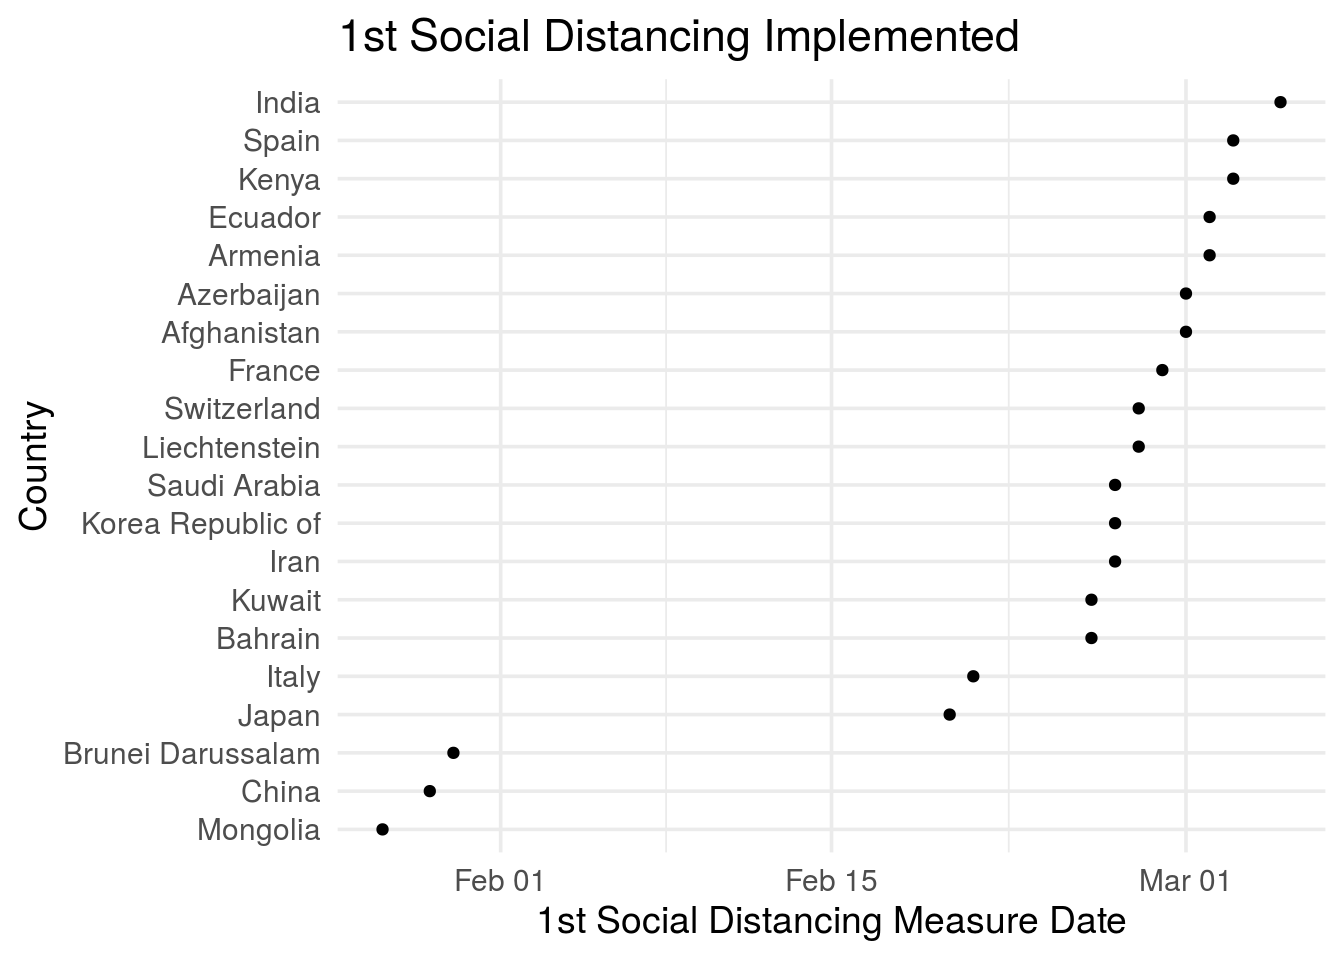
\includegraphics{DataFest_files/figure-latex/top_bottom_10_reactions-1.pdf}

\hypertarget{rvest}{%
\section{RVest}\label{rvest}}

\begin{Shaded}
\begin{Highlighting}[]
\NormalTok{civiqs_poll <-}\StringTok{ "https://civiqs.com/results/approve_president_trump?annotations=true&uncertainty=true&zoomIn=true"}
\NormalTok{html <-}\StringTok{ }\KeywordTok{read_html}\NormalTok{(civiqs_poll)}

\NormalTok{characters <-}\StringTok{ }\KeywordTok{html_text}\NormalTok{(html, }\StringTok{".iLEVuK:nth-child(9) .blyETw:nth-child(1) , .iLEVuK:nth-child(9) .kTXupV:nth-child(1) , .iLEVuK:nth-child(9) .eafFIQ"}\NormalTok{)}

\NormalTok{characters}
\end{Highlighting}
\end{Shaded}

\begin{verbatim}
## [1] "!function(e,p){if(!p.__SV){var o,r,t=window;try{var n,i,a,l=t.location,s=l.hash;n=function(e,t){return(i=e.match(RegExp(t+\"=([^&]*)\")))?i[1]:null},s&&n(s,\"state\")&&(\"mpeditor\"===(a=JSON.parse(decodeURIComponent(n(s,\"state\")))).action&&(t.sessionStorage.setItem(\"_mpcehash\",s),history.replaceState(a.desiredHash||\"\",e.title,l.pathname+l.search)))}catch(e){}(window.mixpanel=p)._i=[],p.init=function(e,t,n){function i(e,t){var n=t.split(\".\");2==n.length&&(e=e[n[0]],t=n[1]),e[t]=function(){e.push([t].concat(Array.prototype.slice.call(arguments,0)))}}var a=p;for(void 0!==n?a=p[n]=[]:n=\"mixpanel\",a.people=a.people||[],a.toString=function(e){var t=\"mixpanel\";return\"mixpanel\"!==n&&(t+=\".\"+n),e||(t+=\" (stub)\"),t},a.people.toString=function(){return a.toString(1)+\".people (stub)\"},o=\"disable time_event track track_pageview track_links track_forms register register_once alias unregister identify name_tag set_config reset people.set people.set_once people.increment people.append people.union people.track_charge people.clear_charges people.delete_user\".split(\" \"),r=0;r<o.length;r++)i(a,o[r]);p._i.push([e,t,n])},p.__SV=1.2,(t=e.createElement(\"script\")).type=\"text/javascript\",t.async=!0,t.src=\"undefined\"!=typeof MIXPANEL_CUSTOM_LIB_URL?MIXPANEL_CUSTOM_LIB_URL:\"file:\"===e.location.protocol&&\"//cdn.mxpnl.com/libs/mixpanel-2-latest.min.js\".match(/^\\/\\//)?\"https://cdn.mxpnl.com/libs/mixpanel-2-latest.min.js\":\"//cdn.mxpnl.com/libs/mixpanel-2-latest.min.js\",(n=e.getElementsByTagName(\"script\")[0]).parentNode.insertBefore(t,n)}}(document,window.mixpanel||[]),mixpanel.init(\"4fe93fbe685935a799cffb6d71db6def\")!function(e,a,t,n,g,c,o){e.GoogleAnalyticsObject=g,e.ga=e.ga||function(){(e.ga.q=e.ga.q||[]).push(arguments)},e.ga.l=1*new Date,c=a.createElement(t),o=a.getElementsByTagName(t)[0],c.async=1,c.src=\"https://www.google-analytics.com/analytics.js\",o.parentNode.insertBefore(c,o)}(window,document,\"script\",0,\"ga\"),ga(\"create\",\"UA-42473732-3\",\"auto\"),ga(\"send\",\"pageview\")Civiqs!function(f){function e(e){for(var r,t,n=e[0],o=e[1],u=e[2],i=0,l=[];i<n.length;i++)t=n[i],c[t]&&l.push(c[t][0]),c[t]=0;for(r in o)Object.prototype.hasOwnProperty.call(o,r)&&(f[r]=o[r]);for(s&&s(e);l.length;)l.shift()();return p.push.apply(p,u||[]),a()}function a(){for(var e,r=0;r<p.length;r++){for(var t=p[r],n=!0,o=1;o<t.length;o++){var u=t[o];0!==c[u]&&(n=!1)}n&&(p.splice(r--,1),e=i(i.s=t[0]))}return e}var t={},c={1:0},p=[];function i(e){if(t[e])return t[e].exports;var r=t[e]={i:e,l:!1,exports:{}};return f[e].call(r.exports,r,r.exports,i),r.l=!0,r.exports}i.m=f,i.c=t,i.d=function(e,r,t){i.o(e,r)||Object.defineProperty(e,r,{enumerable:!0,get:t})},i.r=function(e){\"undefined\"!=typeof Symbol&&Symbol.toStringTag&&Object.defineProperty(e,Symbol.toStringTag,{value:\"Module\"}),Object.defineProperty(e,\"__esModule\",{value:!0})},i.t=function(r,e){if(1&e&&(r=i(r)),8&e)return r;if(4&e&&\"object\"==typeof r&&r&&r.__esModule)return r;var t=Object.create(null);if(i.r(t),Object.defineProperty(t,\"default\",{enumerable:!0,value:r}),2&e&&\"string\"!=typeof r)for(var n in r)i.d(t,n,function(e){return r[e]}.bind(null,n));return t},i.n=function(e){var r=e&&e.__esModule?function(){return e.default}:function(){return e};return i.d(r,\"a\",r),r},i.o=function(e,r){return Object.prototype.hasOwnProperty.call(e,r)},i.p=\"https://results.civiqs.com/\";var r=window.webpackJsonp=window.webpackJsonp||[],n=r.push.bind(r);r.push=e,r=r.slice();for(var o=0;o<r.length;o++)e(r[o]);var s=n;a()}([])"
\end{verbatim}

\begin{Shaded}
\begin{Highlighting}[]
\CommentTok{### Plot of Trump approval rona vs. non-rona}

\NormalTok{covidapproval}\OperatorTok{$}\NormalTok{State =}\StringTok{ }\NormalTok{covidapproval}\OperatorTok{$}\NormalTok{ï..State }

\KeywordTok{ggplot}\NormalTok{(}\DataTypeTok{data =}\NormalTok{ covidapproval, }\KeywordTok{aes}\NormalTok{(}\DataTypeTok{x =} \KeywordTok{reorder}\NormalTok{(State, TrumpCOVID))) }\OperatorTok{+}
\StringTok{  }\KeywordTok{geom_bar}\NormalTok{(}\DataTypeTok{stat =} \StringTok{"identity"}\NormalTok{, }\KeywordTok{aes}\NormalTok{(}\DataTypeTok{y =}\NormalTok{ TrumpCOVID), }\DataTypeTok{fill =} \StringTok{"red"}\NormalTok{, }\DataTypeTok{alpha =} \FloatTok{0.2}\NormalTok{) }\OperatorTok{+}
\StringTok{  }\KeywordTok{geom_point}\NormalTok{(}\DataTypeTok{stat =} \StringTok{"identity"}\NormalTok{, }\KeywordTok{aes}\NormalTok{(}\DataTypeTok{y =}\NormalTok{ Trumpapprov), }\DataTypeTok{color =} \StringTok{"black"}\NormalTok{) }\OperatorTok{+}
\StringTok{  }\KeywordTok{theme}\NormalTok{(}\DataTypeTok{axis.text.x =} \KeywordTok{element_text}\NormalTok{(}\DataTypeTok{angle =} \DecValTok{90}\NormalTok{))}
\end{Highlighting}
\end{Shaded}

\includegraphics{DataFest_files/figure-latex/unnamed-chunk-1-1.pdf}

\end{document}
